\section{Stability Analysis}

With regards to the stability analysis, we aim to try and prove some results on
the "stability function" $R(z)$ as seen in Levecue's \cite{levecue} chapter five
through eight by following the arguments in Staff \cite{staff}.

Suppose we have the following ordinary differential equation:
\begin{equation} \label{eq:lode}
  \begin{cases}
    u' = \mu u, \quad \mu < 0, t > 0 \\
    u(0) = u_0
  \end{cases}
\end{equation}
We would like to analyze the stability of parareal on this system with a 
coarse operator $\coarse$ and a fine operator $\fine$.

\subsection{Deriving a Stability Function}

With respect to Parareal, let's try and write our iteration in the form
$\lambda_n^k = H(n,k)\lambda_0$. Suppose that we have some integrators $\coarse$
and $\fine$, such that they're actually the same method, but with different time
scales. In addition, suppoes that they're iteration can be described by they're
own stability function $R(z)$. Then our parareal iteration goes to:
\begin{align*}
  \lambda_{n+1}^{k+1} & = \coarse(t^{n+1},t^n,\lambda_n^{k+1}) +
  \fine(t^{n+1},t^n,\lambda_n^k) -
  \coarse(t^{n+1},t^n,\lambda_n^k) \\
  & = R(\mu\Delta t)\lambda_n^{k+1} + 
  R(\mu\delta t)^s \lambda_n^k -
  R(\mu\Delta t)\lambda_n^k \\
\end{align*}
where we say $s = \Delta t/ \delta t$, i.e. how many fine steps are needed to
make one coarse step. Combining like terms results in:
\[
  \lambda_{n+1}^{k+1} = 
  R(\mu\Delta t)\lambda_n^{k+1} + 
  \left( R(\mu\delta t)^s - R(\mu\Delta t)\right) \lambda_n^k 
\]
Now, if we were to note the terms on $\lambda$, we note that we have something
very similar to the recurrence relation on combinations $\binom{n}{k} =
\binom{n}{k-1} + \binom{n-1}{k-1}$. Exploiting that relationship, we can unroll
our recursion into:
\[
  \lambda_{n+1}^{k+1} = \left( \sum_{i=0}^k \binom{n}{i} \left[R(\mu \delta t)^s -
    R(\mu \Delta t)\right]^i R(\mu \Delta t)^{n-i} \right) \lambda_0 =
    H(\mu, n,k,\delta t, \Delta t) \lambda_0
\]
We would like to see when it's true that $\abs{H} \leq 1$. As it turns out, this
function is very difficult to analyze by itself, none of my plots of $H$ by
itself generated useful stability regions. Instead we try to analyze this under
a few easy cases, and see exactly how parareal transforms the stability region
of known temporal integrators.

\subsection{Trivial case: $k = 0$}

First, we make a sanity check, suppose we make no Parareal iterations. We would
assume that in this case that the stability function of Parareal should devolve
to the stability function of $\coarse$, since that's the only thing computed.
Indeed:
\begin{align*}
  H & = \left( \sum_{i=0}^0 \binom{n}{i} \left[ R(\mu \delta t)^s -
    R(\mu \Delta t) \right]^i R(\mu \Delta t)^{n-i} \right) \lambda_0 \\
  & = \binom{n}{0} \left[ R(\mu \delta t)^s - R(\mu \Delta t) \right]^0 R(\mu
  \Delta t)^{n} \lambda_0 \\
  & = R(\mu \Delta t)^{n} \lambda_0
\end{align*}
which is precisely the stability function of $\coarse$.

\subsection{Trivial case $\coarse = \fine$.}

Suppose we were to choose $\coarse = \fine$, time scales and all. This implies
that $s = 1$. We would expect that in this case, our parareal algorithm should
result in the stability region of $\coarse$, since the corrector step should
result in a correction of $0$. Indeed we see that all parareal iterations with
$k > 0$ are canceled to zero by the term $[R(\mu \delta t)^s - R(\mu \Delta
t)]$. Otherwise we're just left with $\binom{n}{0} R(\mu \Delta t)^n \lambda_0 =
R(\mu \Delta t)^n \lambda_0$, which is exactly the stability region of
$\coarse$, as expected.

\subsection{Parareal Under Explicit Euler}

The most iconic temporal integrator is the Euler methods, and we would like to
see how Parareal changes they're stability regions.  Suppose now that we are
using explicit Euler for our coarse and fine integrators.  Recall, that this
implies that the stability function for our integrators $\coarse$ and $\fine$
are $(1+z)$ and $(1+z)^s$ respectively, and remember that original the
region of stability for explicit Euler on the given ODE is for $z$ in the unit
disk centered around $-1$. 

Suppose $\fine = \coarse$ but with the time scale squared, i.e. $\delta t =
\Delta t^2$ . So for example, if $\coarse$ has a time step of $1/10$, then
$\fine$ has a time step of $1/100$.  Then, $s = \frac{\Delta t}{\delta t} =
\Delta t^{-1}$. As an example, suppose that $\Delta t = 1/2$. Then $s = 2$, and
(let $z = \Delta t$) our stability region goes to:
\begin{align*}
  H & = \sum_{i=0}^k \binom{n}{i} \left[ R(\mu \delta t)^s -
    R(\mu \Delta t) \right]^i R(\mu \Delta t)^{n-i} \\
  & = \sum_{i=0}^k \binom{n}{i} \left[ (1+\mu z^2)^2 -
    (1+\mu z) \right]^i (1+\mu z)^{n-i} \\
  & = \sum_{i=0}^k \binom{n}{i} 
    \left[ 
      \mu^2 z^4 + 2\mu z^2 - \mu z 
    \right]^i (1+\mu z)^{n-i} \\
  & = \sum_{i=0}^k \binom{n}{i} 
    \left[ 
      \mu z(\mu z^3 + 2 z - 1)
    \right]^i (1+\mu z)^{n-i} \\
\end{align*}
At this point the roots of the cubic are ugly, so I don't take the general case
any further. Now we examine interesting cases under $k$. Recall, by arguments
made above, we already know that $k = 0 \implies$ that we just have stability
region $(1 + \mu z)$. For the following analysis, suppose we take $n = 2$ too.

\subsubsection{One Parareal Iteration: $k = 1$}

Suppose we only make one parareal iteration. Then the above goes to:
\[
  (1 + \mu z)^2 + 2\mu z(\mu z^3 + 2z - 1)(1+\mu z) = (1+\mu z)(2\mu^2 z^4 +
  4\mu z^2  - \mu z + 1)
\]

\subsubsection{Two Parareal Iteration: $k = 2$}

Suppose we make two parareal iteration. This is a little more painful to
compute:
\[
  (1 + \mu z)^2 + 2\mu z(\mu z^3 + 2z - 1)(1+\mu z) + \mu z(\mu z^3 + 2 z - 1) =
  (\mu z^2 + 1)^4
\]
So the stability region $(1 + \mu z)^2$ transformed to $(1 + \mu z^2)^4$ under
two parareal iteration, which is exactly the same region.

\begin{figure}[!htb]
  \centering
  \begin{subfigure}{\textwidth}
    \centering
    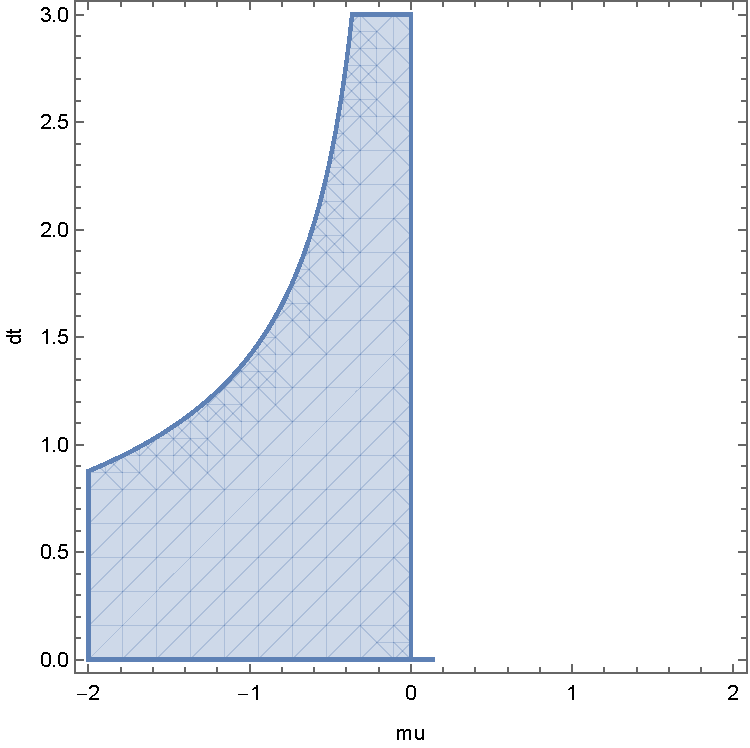
\includegraphics[width=.49\textwidth]
      {./resources/parareal_stability1}
    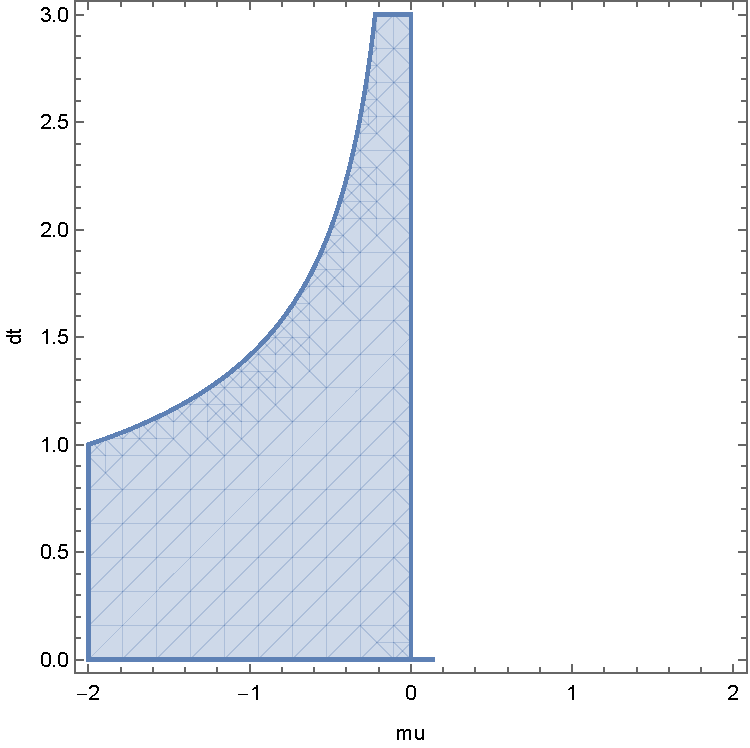
\includegraphics[width=.49\textwidth]
      {./resources/parareal_stability2}
  \end{subfigure}%
  \caption{On the left we have the stability region for $k = 1$, and
  on the right we have it for $k = 2$. It's a little bit difficult to see, but
  for $k = 1$, the stability region is a bit smaller in $\Delta t$, but larger
  in $\mu$.}\label{fig:parareal_stability}
\end{figure}
